\documentclass[14pt]{extarticle}

\usepackage{fontspec}
\setmainfont{Times New Roman}

% размер полей
\usepackage{geometry}
\geometry{a4paper, top=2cm, bottom=2cm, right=1.5cm, left=3cm}

 %debugging
%\usepackage{showframe}

% полуторный интервал
\usepackage{setspace}
\onehalfspacing

% абзацный отступ
\setlength{\parindent}{1.25cm}

% выравнивание текста по ширине
\sloppy

% списки
\usepackage{calc} % арифметические операции с величинами
\usepackage{enumitem}
\setlist{
    nosep,
    leftmargin=0pt,
    itemindent=\parindent + \labelwidth - \labelsep,
}

% подписи к рисункам и таблицам
\usepackage{caption}
\renewcommand{\figurename}{Рисунок}
\renewcommand{\tablename}{Таблица}
\DeclareCaptionFormat{custom}
{
    \textit{#1#2#3}
}
\DeclareCaptionLabelSeparator{custom}{. }
\captionsetup{
    % хз какой это размер - 12 или нет, но выглядит меньше 14
    font=small,
    format=custom,
    labelsep=custom,
}

% картинки
\usepackage{graphicx}

% колонтитулы
\usepackage{fancyhdr}

% картинки и таблицы находятся именно в том месте текста где помещены (атрибут H)
\usepackage{float}

% таблицы
\usepackage{tabularray}

\graphicspath{ {8.2.3/models/} }
\usepackage{hyperref}
\begin{document}
\pagestyle{fancy}
\fancyhead{}
% disable header
\renewcommand{\headrulewidth}{0pt}
\fancyfoot[L]{Дубровских гр 221-361}
\fancyfoot[C]{ЛР 8.2.3}
\fancyfoot[R]{Продажа автотранспорта}
\singlespacing

\newpage
\begin{center}
    Министерство науки и высшего образования Российской Федерации
    Федеральное государственное автономное образовательное учреждение

    высшего образования

    \guillemotleft МОСКОВСКИЙ ПОЛИТЕХНИЧЕСКИЙ УНИВЕРСИТЕТ\guillemotright

    (МОСКОВСКИЙ ПОЛИТЕХ)
\end{center}
\noindent
\bigbreak
\bigbreak
\bigbreak
\bigbreak
\begin{center}
    ЛАБОРАТОРНАЯ РАБОТА 8.2.3

    По курсу Проектирования пользовательских интерфейсов в веб

    \textbf{Разработка пользовательского интерфейса мобильного приложения и прототипа}
    \bigbreak
    \bigbreak
    \bigbreak
    \bigbreak
    ТЕМА

    \guillemotleft\textbf{САЙТ ДЛЯ ПРОДАЖИ И ПОИСКА АВТОМОБИЛЕЙ}\guillemotright
\end{center}
\noindent
\bigbreak
\bigbreak
\bigbreak
\bigbreak
\bigbreak
\bigbreak
\bigbreak
\bigbreak
\bigbreak
\bigbreak
\hfill Выполнил

\hfill Дубровских Никита Евгеньевич

\hfill Группа 221-361
\bigbreak
\bigbreak
\bigbreak
\hfill Проверил

\hfill Натур ВВ
\vfill
\begin{center}
    Москва, 2024
\end{center}
\newpage
\onehalfspacing


\begin{center}
    \textbf{Лабораторная работа 8.2.3}

    \textbf{Разработка пользовательского интерфейса мобильного приложения и прототипа}
\end{center}

\textbf{Цель работы:} спроектировать пользовательский интерфейс мобильного приложения и разработать прототип
\bigskip

\textbf{Задачи:}

\begin{enumerate}
    \item Изучить основы разработки пользовательского интерфейса мобильного приложения
    \item Зафиксировать отличия разработки интерфейсов мобильного приложения и веб-сайта.
    \item Определиться с тематикой и стилем, посмотреть аналоги.
    \item Рассмотреть гайдлайны и UI-kit
    \item Под выбранные тематику и стиль мобильного приложения подобрать контент: шрифтовое оформление, цветовую палитру, изображения.
    \item Продумать пользовательский сценарий и карту мобильного приложения
    \item Определиться с платформой и модульной (колоночной сеткой).
    \item Композиционно выстроить элементы интерфейса страниц мобильного приложения согласно принципам юзабилити, визуальной иерархии, композиции, паттернам, «правилу третей» и правилу «золотого сечения»
    \item При необходимости продумать и разработать онбординг и анимацию
    \item Создать кликабельный прототип мобильного приложения
\end{enumerate}
\bigskip

\textbf{Основные термины}

\begin{itemize}
    \item Пользовательский интерфейс (UI) - визуальный интерфейс, с которым взаимодействует пользователь мобильного приложения.
    \item Прототип - предварительная модель приложения, позволяющая протестировать и визуализировать его функциональность.
    \item Гайдлайны - рекомендации и стандарты по разработке интерфейсов, предоставляемые платформами (например, Apple и Google).
    \item UI-kit - набор элементов пользовательского интерфейса, которые можно использовать при разработке приложений.
    \item Юзабилити - удобство использования приложения, охватывающее доступность, интуитивность и эффективность интерфейса.
    \item Онбординг - процесс введения пользователя в интерфейс приложения с целью облегчения его адаптации.
    \item Визуальная иерархия - принцип организации элементов интерфейса для упрощения восприятия информации пользователем.
    \item Композиция - размещение элементов на экране для создания эстетичного и функционального интерфейса.
    \item Типографика - использование шрифтов и текста в дизайне приложения, включая их размеры и стили.
    \item Цветовая палитра - выбор и сочетание цветов, используемых в интерфейсе.
    \item Модульная сетка - система колонок, помогающая организовать элементы интерфейса в упорядоченном виде.
    \item Кликабельный прототип - интерактивная версия прототипа, позволяющая пользователю взаимодействовать с ним.
\end{itemize}
\bigskip

\textbf{Отличия разработки интерфейсов мобильного приложения и веб-сайта}
\bigskip

1. Платформа и устройство

\begin{itemize}
    \item Мобильное приложение: Разрабатывается для конкретных мобильных операционных систем (iOS, Android). Интерфейс адаптируется к различным экранам и размерам устройств, учитывая особенности сенсорного управления.
    \item Веб-сайт: Доступен через браузер на различных устройствах (десктопы, планшеты, мобильные телефоны). Интерфейс может быть адаптивным (responsive) или адаптированным (adaptive), чтобы подходить для разных экранов.
\end{itemize}

2. Методы взаимодействия

\begin{itemize}
    \item Мобильное приложение: Использует сенсорные экраны, жесты (свайпы, прокрутки, нажатия), что требует других подходов к проектированию кнопок и элементов управления. Элементы интерфейса должны быть достаточно крупными и удобно расположенными для удобства взаимодействия.
    \item Веб-сайт: Основан на взаимодействии с помощью мыши и клавиатуры, что позволяет использовать более мелкие элементы управления и сложные интерфейсы (например, выпадающие меню).
\end{itemize}

3. Доступ к функциям устройства

\begin{itemize}
    \item Мобильное приложение: Может использовать аппаратные функции устройства, такие как GPS, камера, сенсоры (акселерометр, гироскоп) и уведомления. Это открывает новые возможности для взаимодействия и персонализации.
    \item Веб-сайт: Имеет ограниченный доступ к аппаратным функциям устройства. Некоторые функции, такие как GPS, могут быть доступны, но требуют разрешений и работают менее эффективно.
\end{itemize}

4. Пользовательский опыт (UX)

\begin{itemize}
    \item Мобильное приложение: Сфокусирован на быстром и интуитивно понятном доступе к информации и функционалу. Интерфейсы часто требуют меньше текста и больше визуальных элементов, чтобы быть более понятными на маленьких экранах.
    \item Веб-сайт: Может содержать больше информации и более сложные элементы навигации, так как экран больше и взаимодействие происходит через указатель. Пользователи ожидают наличие более обширного контента и навигации.
\end{itemize}

5. Производительность и подключение

\begin{itemize}
    \item Мобильное приложение: Часто требует загрузки и установки на устройство, что может повлиять на производительность и объем памяти. Однако после установки может работать офлайн.
    \item Веб-сайт: Доступен через интернет-браузер и не требует установки, но зависит от качества интернет-соединения и может медленно загружаться.
\end{itemize}

6. Дизайн и стилизация

\begin{itemize}
    \item Мобильное приложение: Использует специфические гайдлайны для каждой платформы (Material Design для Android, Human Interface Guidelines для iOS), чтобы обеспечить консистентность и нативность интерфейса.
    \item Веб-сайт: Может использовать более универсальные подходы к дизайну, однако также должен учитывать кросс-браузерную совместимость и адаптивность.
\end{itemize}

7. Обновления и поддержка

\begin{itemize}
    \item Мобильное приложение: Требует обновлений через магазины приложений, что может потребовать больше времени на внедрение новых функций и исправления ошибок.
    \item Веб-сайт: Мгновенно обновляется на сервере, что позволяет пользователям видеть изменения без необходимости обновления страницы или приложения.
\end{itemize}
\bigskip

\textbf{Паттерны}

\noindent
\begin{minipage}{\linewidth}
    \fbox{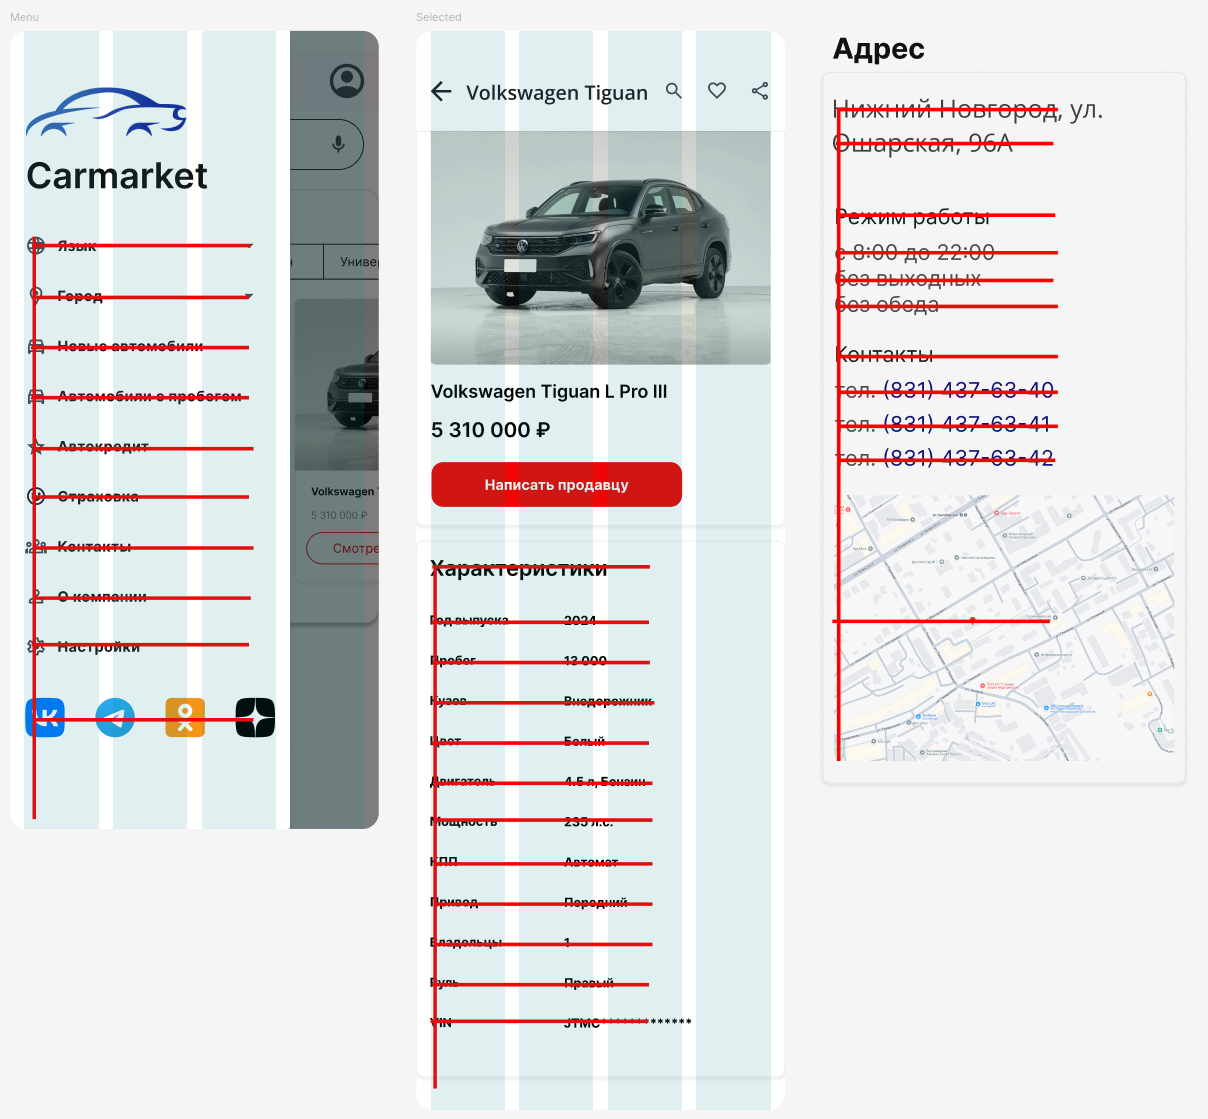
\includegraphics[width=\linewidth]{f}}
    \captionof{figure}{F-паттерн}
\end{minipage}
\bigskip

\textbf{Палитра}

\noindent
\begin{minipage}{\linewidth}
    \fbox{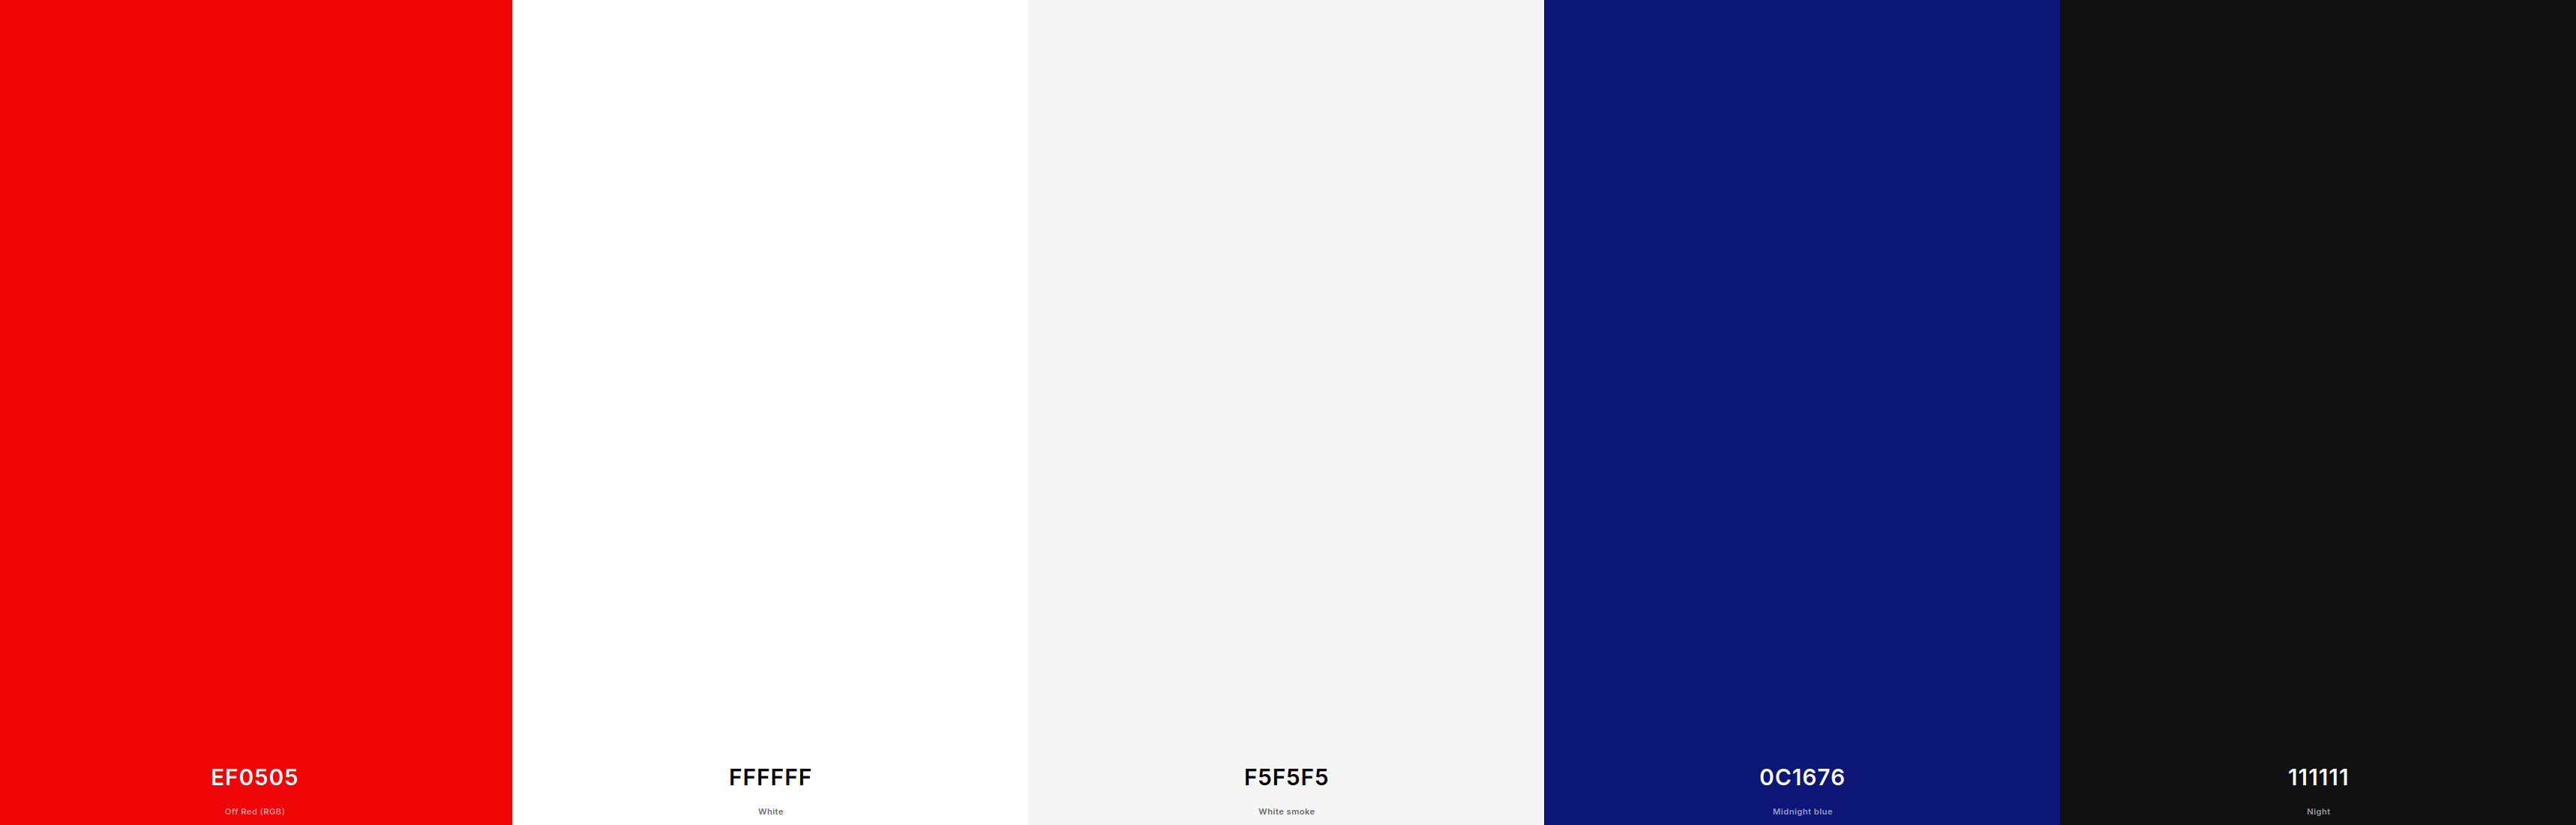
\includegraphics[width=\linewidth]{coolors5}}
    \captionof{figure}{Палитра}
\end{minipage}
\bigskip

\textbf{Типографика}

\noindent
\begin{minipage}{\linewidth}
    \fbox{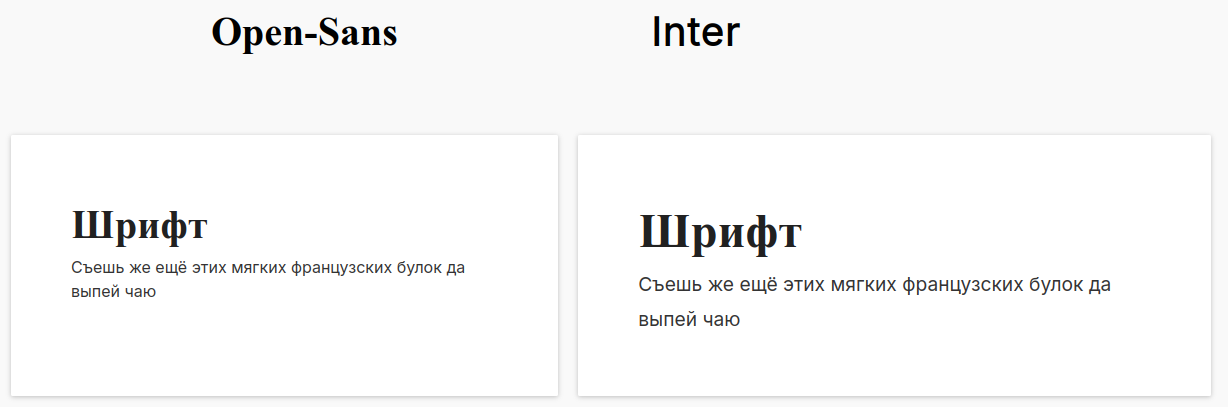
\includegraphics[width=\linewidth]{mix}}
    \captionof{figure}{Шрифты}
\end{minipage}
\bigskip

\textbf{Сетка}

\noindent
\begin{minipage}{\linewidth}
    \fbox{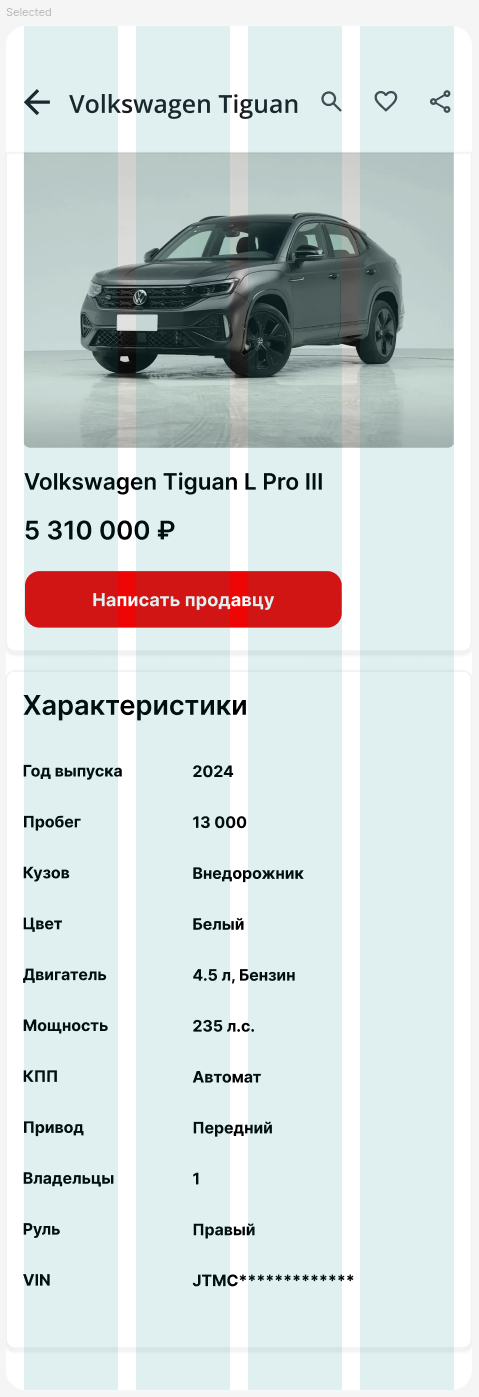
\includegraphics[scale=0.5]{grid}}
    \captionof{figure}{Сетка}
\end{minipage}
\bigskip

\textbf{Гайдлайны и UI-кит}
\bigskip

В качестве гайдлайна и UI-кита был выбран Material Design 3:

\begin{table}[H]
    \small
    \setstretch{1}
    \begin{tabular}{|p{3cm}|p{5cm}|p{6cm}|}
\hline
\textbf{Компонент} & \textbf{Описание} & \textbf{Рекомендации} \\
\hline
Цвет & Цветовая палитра Material Design включает основные и акцентные цвета. & Используйте яркие, насыщенные цвета для акцентов, приглушенные для фона. Цвета должны быть доступными для всех пользователей. \\
\hline
Типографика & Material использует набор шрифтов, в основном Roboto и Noto. & Стремитесь к ясности и читаемости. Размеры шрифтов от 12 до 96 px для различных уровней иерархии. \\
\hline
Иконки & Простые, монотонные, легко читаемые иконки с четким значением. & Размер иконок от 18 до 48 dp. Используйте Material Icons или их аналоги. \\
\hline
Отступы и сетка & Сетка и отступы помогают организовать пространство, создавая гармоничную структуру. & Стандартный отступ — 8 dp. Сетки 4 и 8 dp обеспечивают аккуратное расположение элементов. \\
\hline
Карточки & Карточки группируют информацию и действия для отдельной темы. & Используйте тени и закругленные углы. Размеры иерархичны и зависят от контекста. \\
\hline
Кнопки & Кнопки используют понятные действия и предлагают кликать по ним. & Основные кнопки – акцентные цвета, а второстепенные – приглушенные. Закруглённые углы улучшают восприятие. \\
\hline
Анимация и переходы & Анимации добавляют интерактивности и помогают пользователям понять результаты своих действий. & Анимации должны быть короткими (до 300 мс) и поддерживать естественность движений. \\
\hline
Взаимодействие & Касания, жесты и поведение взаимодействий стандартизированы. & Минимальный размер для кликабельных областей – 48x48 dp. Жесты должны быть интуитивными. \\
\hline
Поверхности и слои & Система поверхностей основана на Z-оси, что помогает организовать слои информации. & Используйте тени и высоту для обозначения слоев, акцентируя важные элементы. \\
\hline
Состояния элементов & Состояния (нажато, наведено, отключено) помогают пользователям понять текущую доступность или состояние элементов интерфейса. & Обозначайте состояния с помощью цветов и тени. Отключенные элементы должны выглядеть приглушённо и быть неподвижны. \\
\hline
Форма элементов & Закругленные углы и плавные переходы делают интерфейс более дружественным и современным. & Рекомендуется закругление от 4 до 16 dp в зависимости от компонента. \\
\hline
\end{tabular}
\end{table}

\noindent
\begin{minipage}{\linewidth}
    \fbox{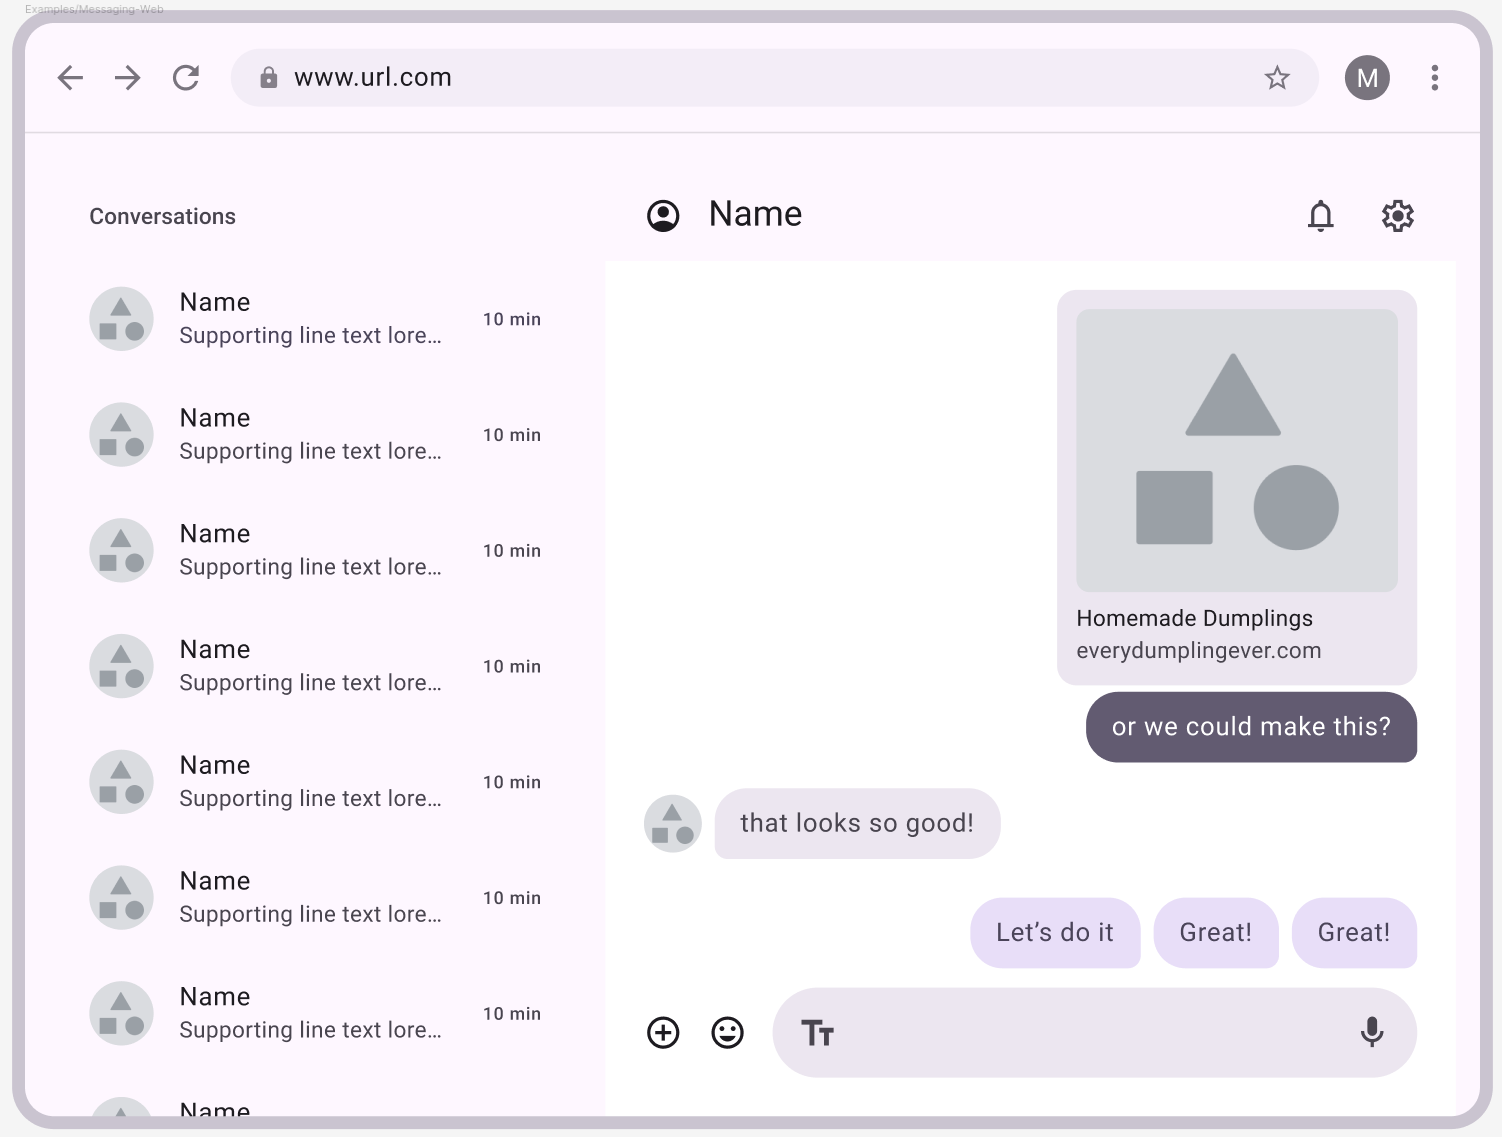
\includegraphics[width=\linewidth]{m3_1}}
\end{minipage}
\bigskip

\noindent
\begin{minipage}{\linewidth}
    \fbox{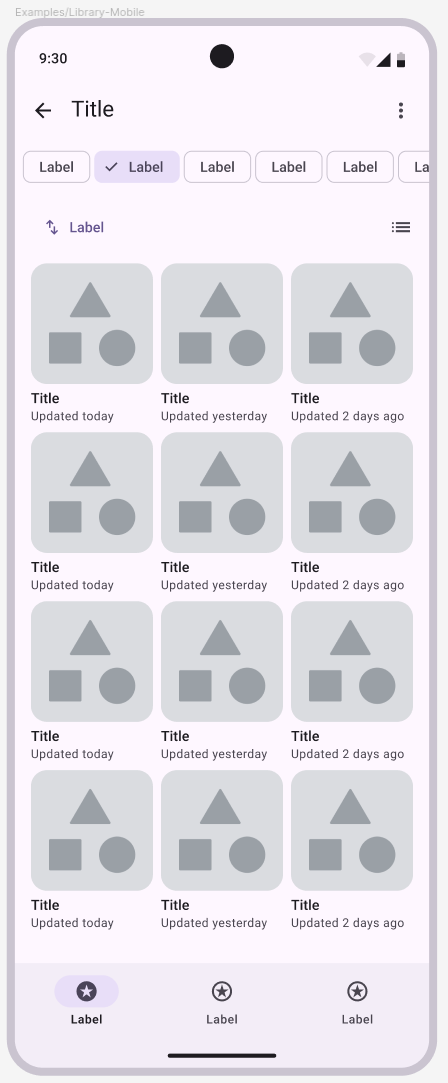
\includegraphics[scale=0.55]{m3_2}}
\end{minipage}
\bigskip

\noindent
\begin{minipage}{\linewidth}
    \fbox{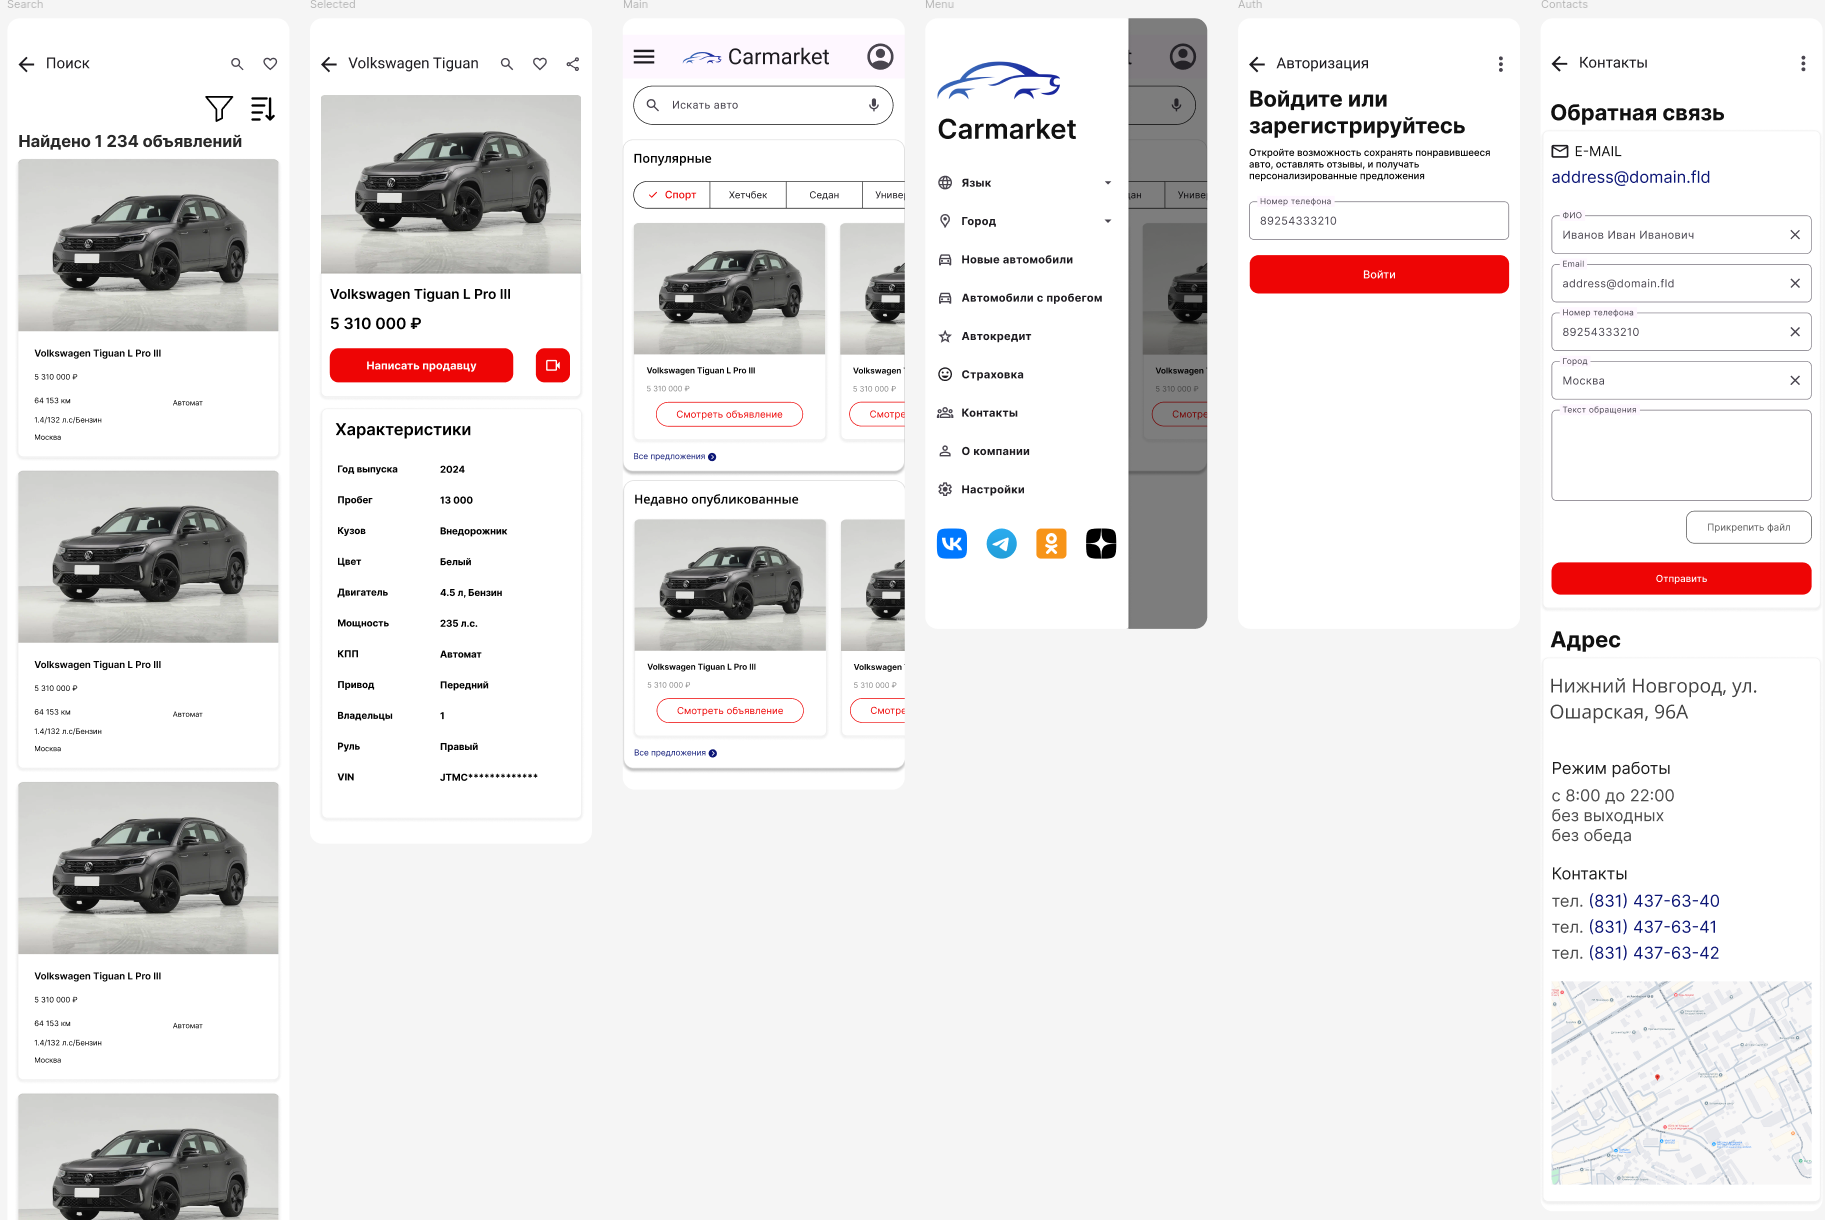
\includegraphics[width=\linewidth]{my1}}
\end{minipage}
\bigskip

\noindent
\begin{minipage}{\linewidth}
    \fbox{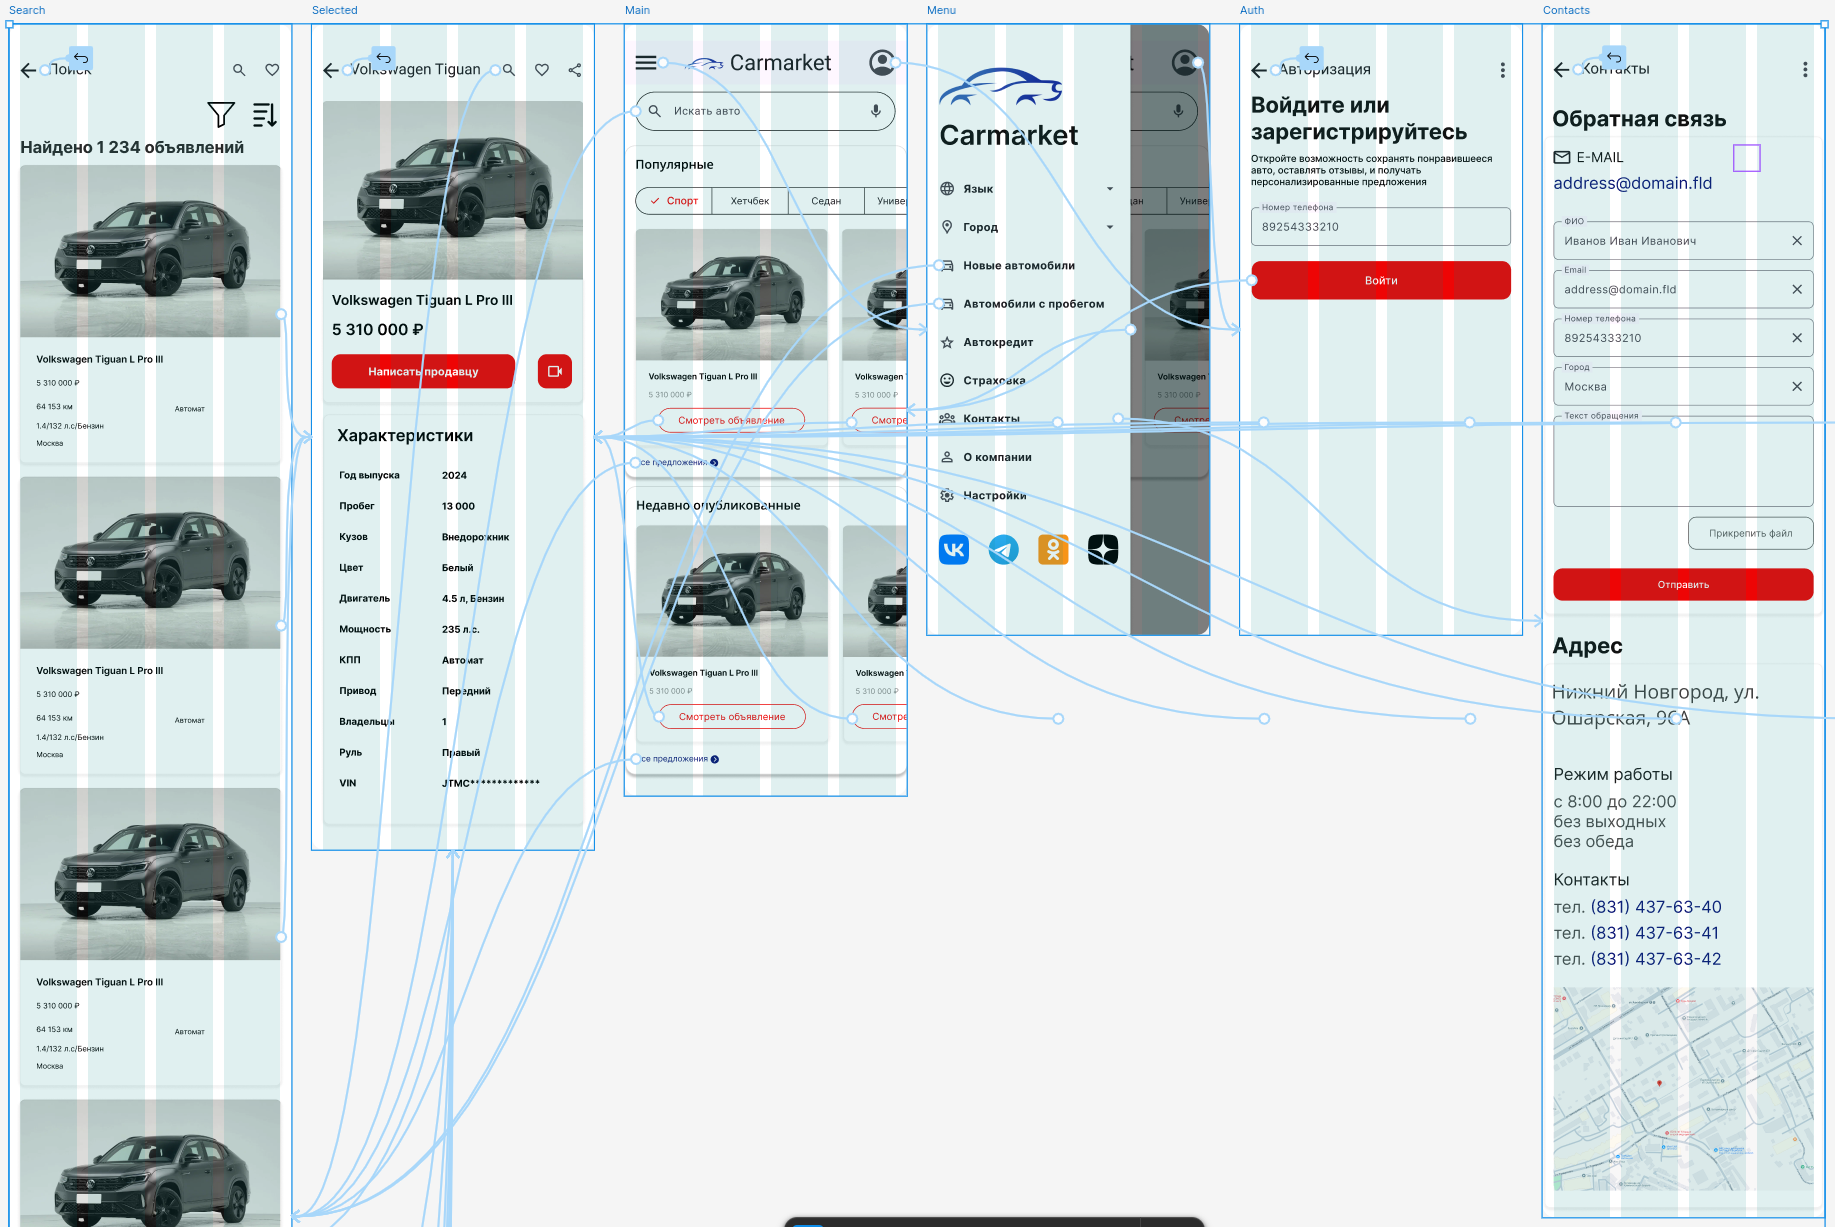
\includegraphics[width=\linewidth]{my2}}
\end{minipage}
\bigskip

\noindent
\begin{minipage}{\linewidth}
    \centering
    \fbox{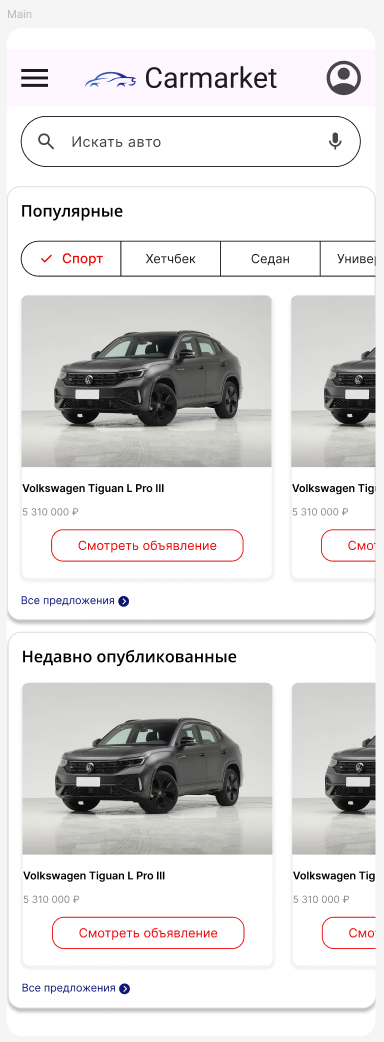
\includegraphics[scale=0.5]{my5}}
    \fbox{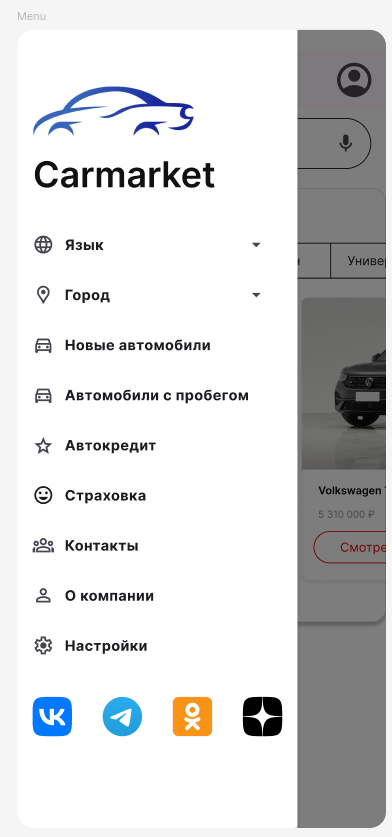
\includegraphics[scale=0.5]{my6}}
\end{minipage}
\bigskip

\noindent
\begin{minipage}{\linewidth}
    \centering
    \fbox{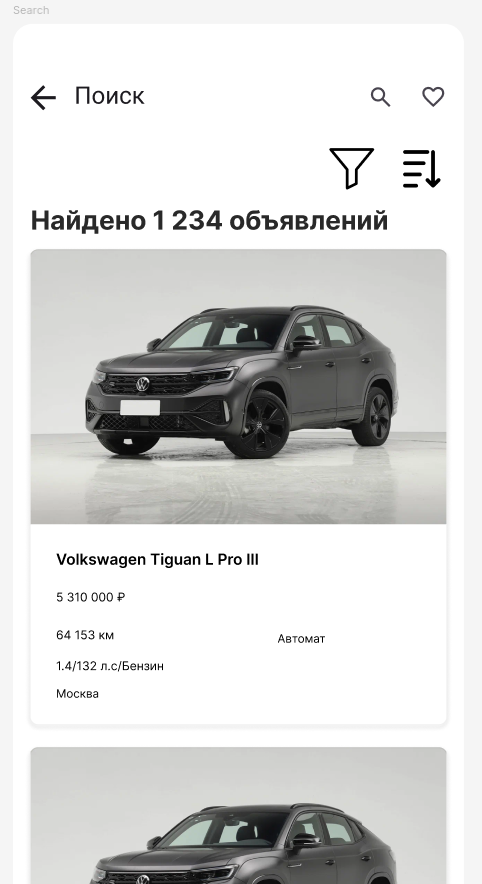
\includegraphics[scale=0.5]{my3}}
    \fbox{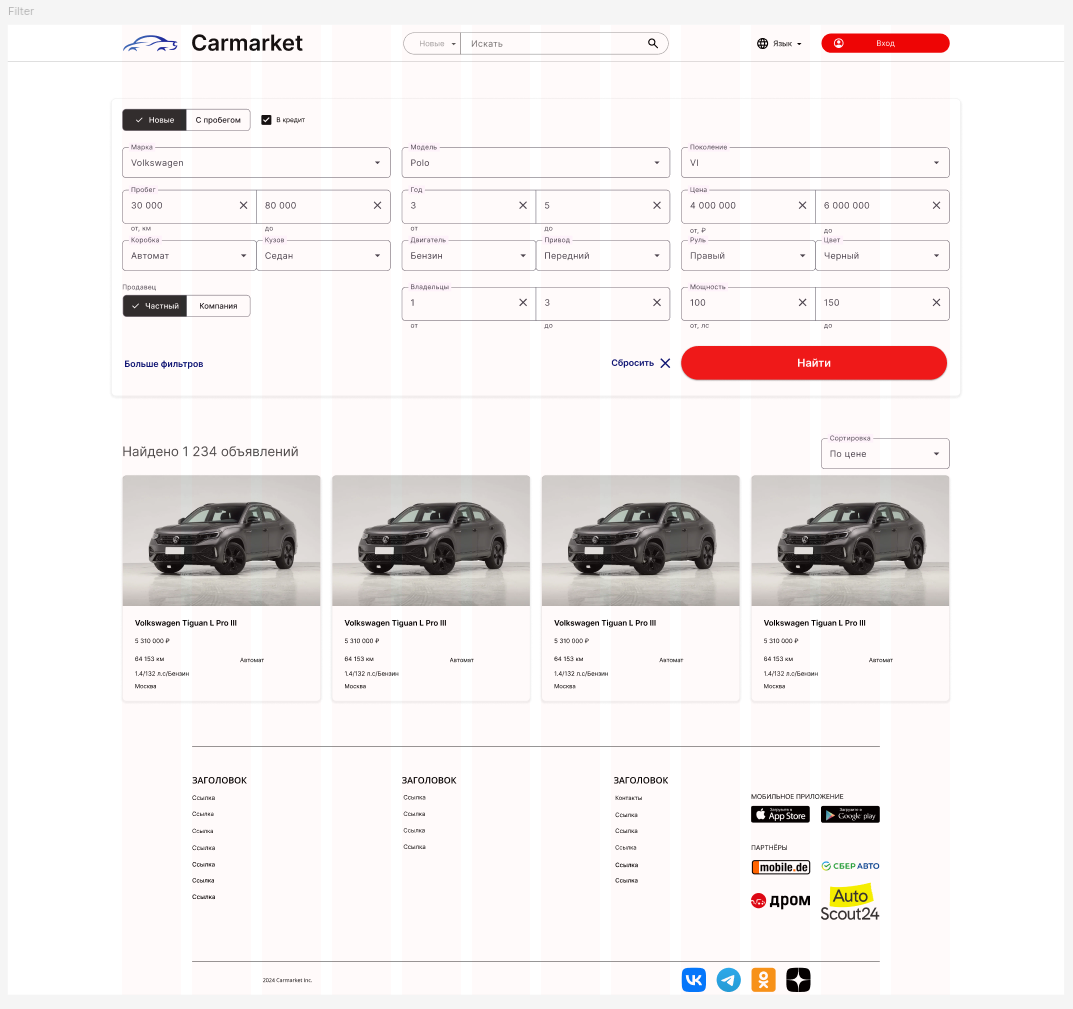
\includegraphics[scale=0.5]{my4}}
\end{minipage}
\bigskip

\noindent
\begin{minipage}{\linewidth}
    \centering
    \fbox{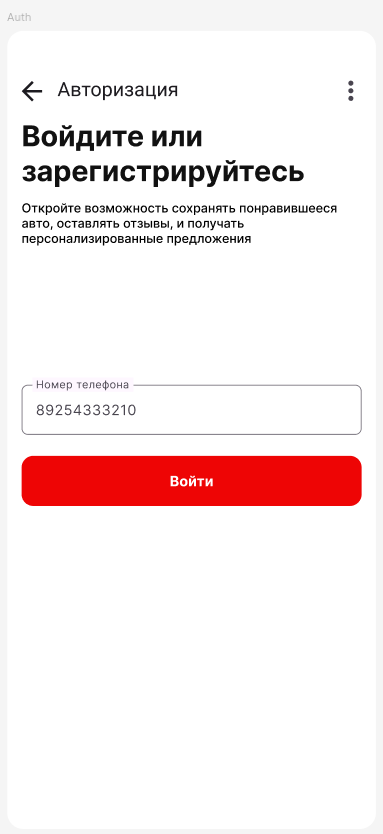
\includegraphics[scale=0.5]{my7}}
    \fbox{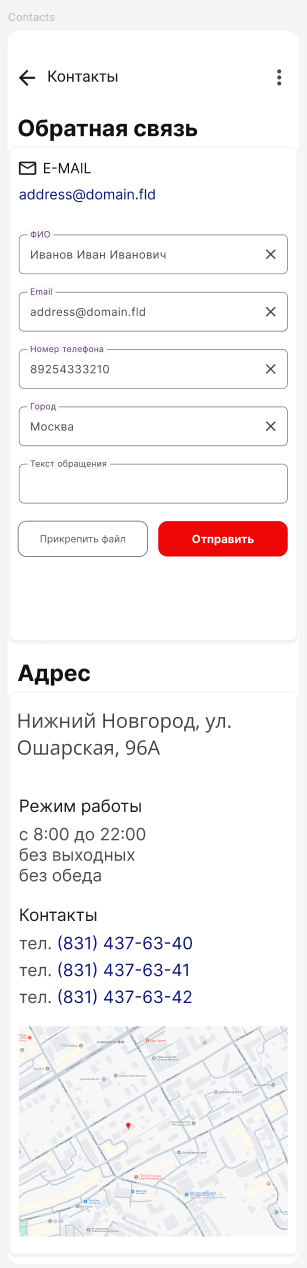
\includegraphics[scale=0.5]{my8}}
\end{minipage}
\bigskip

\textbf{Ссылка:}

\url{https://www.figma.com/design/25STw8qqDFUKFnCIDQb1ri/PPI?node-id=0-1&t=Hg1oP3IEn46EtUel-1}
\bigskip
\bigskip

\textbf{Контрольные вопросы и ответы}

\begin{enumerate}
    \item Что такое мобильное приложение? Цели и задачи UX моб-приложения.

    Мобильное приложение — это программное обеспечение, разработанное для работы на мобильных устройствах, таких как смартфоны и планшеты. Цели UX моб-приложения включают создание интуитивно понятного, удобного и приятного пользовательского опыта, повышение удовлетворенности пользователей и увеличение их вовлеченности. Задачи могут включать изучение потребностей пользователей, проектирование интерфейсов, проведение тестирования и итерационное улучшение.

    \item Специфика разработки интерфейса мобильного приложения. Гайдлайны.

    Специфика разработки интерфейса мобильного приложения заключается в необходимости учитывать ограниченные размеры экранов, различные разрешения и ориентации устройств, а также особенности взаимодействия (сенсорное управление). Гайдлайны, такие как Material Design от Google и Human Interface Guidelines от Apple, предоставляют рекомендации по созданию удобных интерфейсов, включая элементы дизайна, навигацию, типографику и цветовые палитры.

    \item Юзабилити мобильного приложения и паттерны использования.

    Юзабилити мобильного приложения — это мера его удобства и эффективности для пользователя. Ключевые паттерны использования включают принцип "пальца" (размещение элементов управления в пределах легкой досягаемости), использование кнопок вместо ссылок для повышения кликабельности и внедрение привычных жестов (свайп, прокрутка) для навигации.

    \item Специфика подбора контента мобильного приложения.

    Подбор контента для мобильного приложения должен учитывать его легкость восприятия и доступность. Это включает использование кратких текстов, визуально привлекательных изображений и интуитивно понятных иконок. Контент должен быть адаптирован для мобильного формата, чтобы избегать перегруженности экрана и обеспечить четкость информации.

    \item Принципы визуальной иерархии элементов интерфейса информационной системы - мобильного приложения.

    Принципы визуальной иерархии включают использование размера, цвета, контраста и расположения для создания ясного порядка важности элементов. Наиболее важные элементы должны быть выделены (например, через размер или цвет), чтобы пользователь мог легко идентифицировать их и следовать логике приложения. Правило третей и правило "золотого сечения" также помогают в создании сбалансированных композиций.

    \item Что такое онбординг? Цель, задачи, принципы.

    Онбординг — это процесс введения пользователя в функционал приложения, целью которого является облегчение его адаптации. Задачи онбординга включают объяснение основных функций, привлечение внимания пользователя к ключевым особенностям и повышение лояльности. Основные принципы онбординга включают краткость, визуальную привлекательность (использование иллюстраций и анимаций), возможность пропуска и предоставление прогресс-баров, чтобы пользователи могли видеть, сколько шагов осталось до завершения.
\end{enumerate}

\end{document}
